
%%%%%%%%%% Conference Latex Template for the university center of Tipaza - Algeria
%%%%%%%%%% created by F.CHABNI




\documentclass{report}
\usepackage{ctex}
\usepackage{geometry}
\usepackage{graphicx}
\usepackage{amsmath}
\usepackage{cite}
\usepackage{subcaption}
\usepackage{booktabs}
\usepackage{multirow}
% \usepackage{graphicx}
\usepackage[table,xcdraw]{xcolor}
\title{自主移动车文献综述和原型设计}
\author{邱璟祎, 周俊豪, 张峻瑜\\
  (按姓名首字母排序)
}
\geometry{a4paper,scale=0.8}
\begin{document}
\maketitle
\tableofcontents
\newpage
\chapter{引言}
在当今快速发展的科技时代,自动化和智能化已成为工业和日常生活领域的关键趋势。智能小车,作为自动化物流系统中的重要组成部分,其发展和应用备受关注,本课程中的AGV很好地迎合了时代的这一需求。为完成本课程的任务,本文将从课程任务入手,分析各个板块需要完成的任务,并通过文献综述梳理这些任务已有的解决方法,从而在最后给出初步的原理方案设计。
本文中所实现的智能小车指能够自主移动并实现在循迹场景与避障场景中自主完成抓取、运输和卸载货物工作的AGV小车。在对智能小车任务进行需求分析与任务分解后,本文将从机械结构、循迹算法和避障算法三个方面进行文献调研并综述,总结和评估这些领域的现有技术和方法,探索它们在智能小车设计中的应用潜力和局限性。
在广泛调研的基础上,本文将结合需求分析和文献综述的结果,提出一套初步的原理方案设计。该方案将涵盖智能小车的机械结构、测量方法、循迹和避障的算法、数据通信和驱动等。此外,我们还将讨论该方案的可行性和潜在的技术挑战。
通过本文的研究,我们期望为我们课程智能小车的设计提供有价值的参考和指导,也希望能为市场上的智能小车的设计提供一些思路,推动自动化物流技术的进步,为工业自动化和智能运输系统的发展做出贡献。


\chapter{需求分析}
课程任务为:设计并实现一个机电系统,按照规定路线,在2种不同场地,将指定物品从一个指定位置运输到另一指定位置。,两种场地分别需要实现循迹和避障的功能。为了完成这个任务,将任务分解为机械结构、电气、测量、算法和系统软件五个方面的内容。
\section{机械结构}
\label{sec:label}
\subsection{车体结构}
\label{subsec:label}
\begin{enumerate}
\item 整体尺寸:避障部分场地的障碍物间距不小于350mm,故小车的整体尺寸应当小于该距离。
\item 驱动与转弯方式:驱动方式可以选择轮式或者履带式,转弯方式可以采用差速转向或者麦克纳姆轮转向。
  \item 车体空间结构:车上需要装载驱动电机、控制板、传感器等元件以及电子线路,可以考虑设计多层结构,同时需要考虑重心的稳定性和小车的承重性能。
\end{enumerate}
\subsection{抓取机构}
\label{subsec:label}
\begin{enumerate}
\item 机械爪及舵机:货物尺寸为直径30mm,高40mm,其重量为50g,因此抓取结构中的机械爪需与货物尺寸相匹配,且相应舵机需要有足够的力矩。
  \item 抓取结构大小与工作空间:因小车本身体积有限,因此抓取结构不应过大。除此之外,还需考虑抓取结构的工作空间,如不能遮挡摄像头视野等。
  \end{enumerate}
  \newpage
\section{电气}
\label{subsec:label}
\subsection{控制器硬件}
\label{subsec:label}
常用的包括编程调试方便,主要串行执行的CPU和并发速度快,可靠性好,调试困难的FPGA,可以根据功能需求、计算能力等方面的约束进行选取。
\subsection{电机与驱动}
\label{subsec:label}
常用的驱动电机包括航模电机和直流电机等,需要根据驱动力要求、电路负载要求等进行选取。
\subsection{电源}
\label{subsec:label}
单片机、电机、舵机等不同元器件的所需电压不同,需要进行相应的电源与二次电源的选择,具体选择将在原理方案设计部分确定。
\subsection{通讯}
\label{subsec:label}
需要实现的数据通讯任务包括实时图像、指令数据、状态参数和舵机命令等,可以采用USB数据线的有线通讯方式或者蓝牙等无线通讯方式,具体选择需要根据传输数据量、数据传输延时和硬件接口等因素确定。
\section{测量}
\label{sec:label}
需要传感器传回的信息主要包括图像灰度、距离、小车自身的位置和姿态等等,可能需要红外传感器、超声传感器、线阵CCD传感器、里程计和陀螺仪等,需要根据需求进行选取,同时要和车体结构相匹配。
\section{算法}
\label{sec:label}
循迹和避障的算法现有的文献和其他资料都有很多内容,将在后面文献综述部分加以阐述,并在设计部分进行选择。

\section{系统软件}
\label{sec:label}
系统软件需要根据功能和算法进行划分,并且和实际硬件进行对应,从而实现各个模块之间的交互。


\chapter{自主移动车文献综述}
\label{sec:label}


\section{机械设计研究综述}
\subsection{运动方式}
\label{subsec:label}
目前自主移动车的运动方式主要分为轮式和履带式,下面将分别论述这两种方式的特点。
\subsubsection{轮式运动}
\label{subsec:label}
轮式运动是最常见的自主移动车的运动方式,其特点是使用一组或多组轮子进行移动,可以采用常规的轮胎或全向轮设计,适用于平坦、结构简单的环境,灵活程度比较高,结构简单、可控性强、安全性好。按照驱动方式进行分类又可以分为单驱轮式、双驱轮式和多驱轮式。单驱轮式通常适用于三轮式AGV,双驱轮式则通常适用于四轮式AGV,这两类驱动方式的特点是整个AGV只有一部分车轮具有驱动力,可以减少驱动电机的数量,减少车体重量,节约内部空间;但采用这类驱动方式的小车往往由于配重不均匀会出现非驱动轮一侧抓地力不足的问题,小车转向容易出现问题。多驱轮式的AGV的所有车轮都和驱动电机相连,驱动能力更强,配重更加均匀,但是灵活性有所降低。
\subsubsection{履带式运动}
\label{subsec:label}
履带式运动的AGV对地面的单位压力小,摩擦力较大,抓地力较好,适合在雪地、山坡等比较恶劣的地面环境下工作,能承受比较大的负载,但是成本比轮式AGV高很多,速度比较慢。
\newpage
\subsection{转向方式}
\label{subsec:label}
目前已有的AGV中,转向方式大部分都可以归结为差速转向和麦克纳姆轮转向两大类,下面将分别进行叙述
\subsubsection{差速转向\cite{chasu}}
\label{subsec:label}
假定前轮和后轮都是驱动轮,则参考阿克曼(Ackerman)转向几何学原理,即在汽车转向时4个轮胎都近似围绕一个中心点旋转以保证汽车的行驶稳定性。把汽车的形心作为质心,并且忽略路面情况变化等的影响,可得出四轮驱动差速转向小车的运动学模型如下图所示。
\begin{figure}[ht]
  \centering
  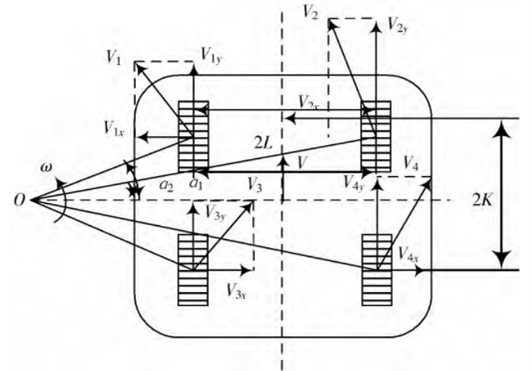
\includegraphics[width=0.5\textwidth]{figures/chasu.png}
  \caption{差速转向受力分析}
\end{figure}
$\alpha_1$和$\alpha_2$分别为前左轮和后左轮,前右轮和右轮的转角;2L 为左右轮距离; 2K 为前后轮轴距;$v$和$\omega$分别为车子质心的线速度和角速度,$V_1,V_2,V_3,V_4$分别为各个轮中心的实际运动方向。由图 可以得出各速度和转角的关系:
\[\begin{gathered}
V_{1}=\omega R_{1}=\omega\frac{K}{sin\alpha_{1}}\leftarrow \\
V_{2}=\omega R_{2}=\omega\frac{K}{sin\alpha_{2}}\leftarrow \\
V_{3}=V_{1}=\omega\frac{K}{sin\alpha_{1}}\leftarrow \\
V_{4}=V_{2}=\omega\frac{K}{sin\alpha_{2}}\leftarrow \\
V_{1y}=V_{1}cos\alpha_{1}= \omega\frac{K}{tan\alpha_{1}}=\omega(R-L)^{\leftrightarrow}\\
V_{2y}=V_{2}cos\alpha_{2}= \omega\frac{K}{tan\alpha_{2}}=\omega(R+L)^{\leftrightarrow}\\
V_{3y}=V_{3}cos\alpha_{1}= \omega\frac{K}{tan\alpha_{1}}=\omega(R-L)^{\leftrightarrow}\\
V_{4y}=V_{4}cos\alpha_{2}= \omega\frac{K}{tan\alpha_{2}}=\omega(R+L)^{\leftrightarrow}
\end{gathered}\]
式中$R=\frac v\omega $。

则电机的角速度为:$\omega_n=\frac{V_{ny}i}r,n=1,2,3,4$

式中$i$为减速器的减速比,$r$为车轮半径。


\subsubsection{麦克纳姆轮转向\cite{mac}}
\label{subsec:label}
麦克纳姆轮移动平台具有平面上3个自由度的移动能力,依靠4个轮子各自不同转速的相互配合来实现全向移动,每一个轮子的运动都对整体的运动方向和速度大小有着很大的贡献。麦克纳姆轮它与普通轮之间的主要区别就在于它的圆周上分布有若干数量的辊子,这些辊子的轴线与轮子的轴线呈一定的夹角(如45°),辊子的外廓线所形成的包络面和轮的原始圆周面重合,这样保证了辊子能与地面一直保持接触这些辊子还可以自由转动,这使得轮子只受到地面对辊子轴向上的力,而地面对辊子的圆周力则变为了滚动摩擦,可以近似看为零。因此,轮子与地面的接触力不再是沿轮子的圆周方向,而是与它呈一定的夹角,所以这种轮子可以在一个方向上受到摩擦力的驱动,而在另一个方向上自由移动。由4个这样的轮子便可以组合出不同的受力情况,从而使移动平台可以实现平面上3个自由度的移动。


用$R$表示全向轮轴心到轮外廓圆周面的距离即轮的半径;$V_i$表示第$i$轮的速度;$\alpha$表示辊子轴线与全向轮轴线夹角;$\omega_i$表示全向轮绕轮轴的转速;i=1,2,3,4,分别代表左前轮、右前轮、左后轮、右后轮。联立可得矩阵方程:
\[ V_i=\begin{pmatrix}R\\4\end{pmatrix}\begin{bmatrix}1&1&1&1\\\tan\alpha&-\tan\alpha&-\tan\alpha&\tan\alpha\\-\frac{1}{l_0}&\frac{1}{l_0}&-\frac{1}{l_0}&\frac{1}{l_0}\end{bmatrix}\begin{bmatrix}\omega_1\\\omega_2\\\omega_3\\\omega_4\end{bmatrix}\leftarrow  \]
式中$l_0=$W+ Lcos$\alpha$,其中 W 为移动平台宽度,L 为其前后轮轴距;而$\alpha$取
$45^{\circ}$,其正负号已被提出,不再区分正负。逆运动学方程为:
\[\begin{bmatrix}\omega_1\\\omega_2\\\omega_3\\\omega_4\end{bmatrix}=\text{K}\begin{bmatrix}V_y\\V_x\\\omega\end{bmatrix}=\begin{pmatrix}\frac{1}{R}\end{pmatrix}\begin{bmatrix}1&cot\alpha&-l_0\\1&-cot\alpha&l_0\\1&-cot\alpha&-l_0\\1&cot\alpha&l_0\end{bmatrix}\begin{bmatrix}V_y\\V_x\\\omega\end{bmatrix}\leftarrow \]
总的来说,麦克纳姆轮转向具有高效率、高灵活性的特点。
\begin{figure}[ht]
  \centering
  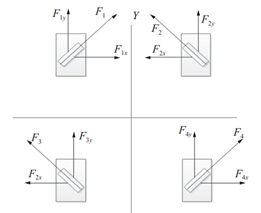
\includegraphics[width=0.5\textwidth]{figures/mac.png}
  \caption{麦克纳姆轮受力分析 }
\end{figure}
\subsection{抓取机构}
\label{subsec:label}
机械臂末端的抓取机构可以采用机械手爪、吸盘和仿生结构三种形式,它们具体的特点如下:
\subsubsection{机械手爪}
\label{subsec:label}
机械手爪按照驱动方式不同可以分为气动驱动、电动驱动、液压驱动、电磁驱动和热驱动五种方式。气动驱动使用压缩空气来控制手爪的开合,成本较低,响应速度快,但是需要压缩空气源,且控制精度相对较低。电动驱动使用电机作为动力源,通过齿轮、皮带或丝杠等机械结构传递动力,控制精度高,力矩输出稳定,但是结构可能较为复杂,成本相对较高。液压驱动利用液压系统产生的动力来驱动手爪,可以产生较大的力,适合重载应用,但是需要液压泵和管路系统,维护成本较高。电磁驱动通过电磁铁产生的磁力来控制手爪的动作,响应速度快,结构简单,但是力量输出可能受限于磁场强度。热驱动利用热胀冷缩的原理来驱动手爪,可以实现柔性抓取,但是响应速度慢,适用范围有限。

\subsubsection{吸盘}
\label{subsec:label}
吸盘可以分为磁力吸盘和真空吸盘两大类。磁力吸盘的体积小,自重轻,吸持力强,广泛应用于钢铁、机械加工、模具、仓库等搬运吊装过程中对块状、圆柱形导磁性钢铁材料工件的连接,可大大提高工件装卸、搬运的效率,但是对所抓取的物品有磁性的要求。真空吸盘原理简单,操作相对容易,但前提是要保证所抓取物品表面足够平整光滑,此外还需要注意对于吸盘盘面的清洁与保护,防止污渍与腐蚀,对于后期维护保养的要求较高。
\subsubsection{仿生结构}
\label{subsec:label}
面对外形较为复杂的物品,可以采用多指灵巧手的仿生结构作为夹持机构。在众多仿生结构中,人形手模仿人类手的外形和运动自由度,通常具有多个关节和独立运动的手指,可以实现复杂的抓取动作,如捏取、旋转和握持,适用于需要高度灵活性和精准控制的应用场景。柔性夹持器采用柔软材料制成,例如硅胶或弹性聚合物,可以根据物体的形状和尺寸进行自适应的夹持,能够温和地处理各种形状的物体,腱驱动手使用类似于人类手臂的腱结构来驱动手指的运动,通过线缆或弹性材料控制手指的张合,提供较好的力量和运动控制,可以实现较强的夹持力和灵活的手指运动。不完全驱动手的手指之间可能共享某些驱动元件,这种设计可以减少驱动部件的数量,提高了系统的可靠性和节省成本。生物启发自适应夹持器借鉴动物或昆虫的夹持机制,如螯虎或章鱼的吸盘结构,实现了在不同形状和尺寸的物体上的高效夹持能力和自适应性。

\newpage
\section{循迹研究综述}
\subsection{传统而有效的方法\cite{intro2023robot}}
\label{subsec:label}
\subsubsection{传感器:红外传感器、光敏电阻等}
\label{subsec:label}
红外传感器、光敏电阻等传感器实际上提供的传感能力是同质化的,此处以红外传感器为例介绍传统方法所用的传感器。

红外传感器是各种机器人比赛中最常见的传感设备。红外传感器可以发射红外光并接收反射光,根据反射光的强度输出电压。输出电压在经过有着固定基准值的电压比较器处理后将输出逻辑电平,便于控制器处理。
\begin{figure}[ht]
  \centering
  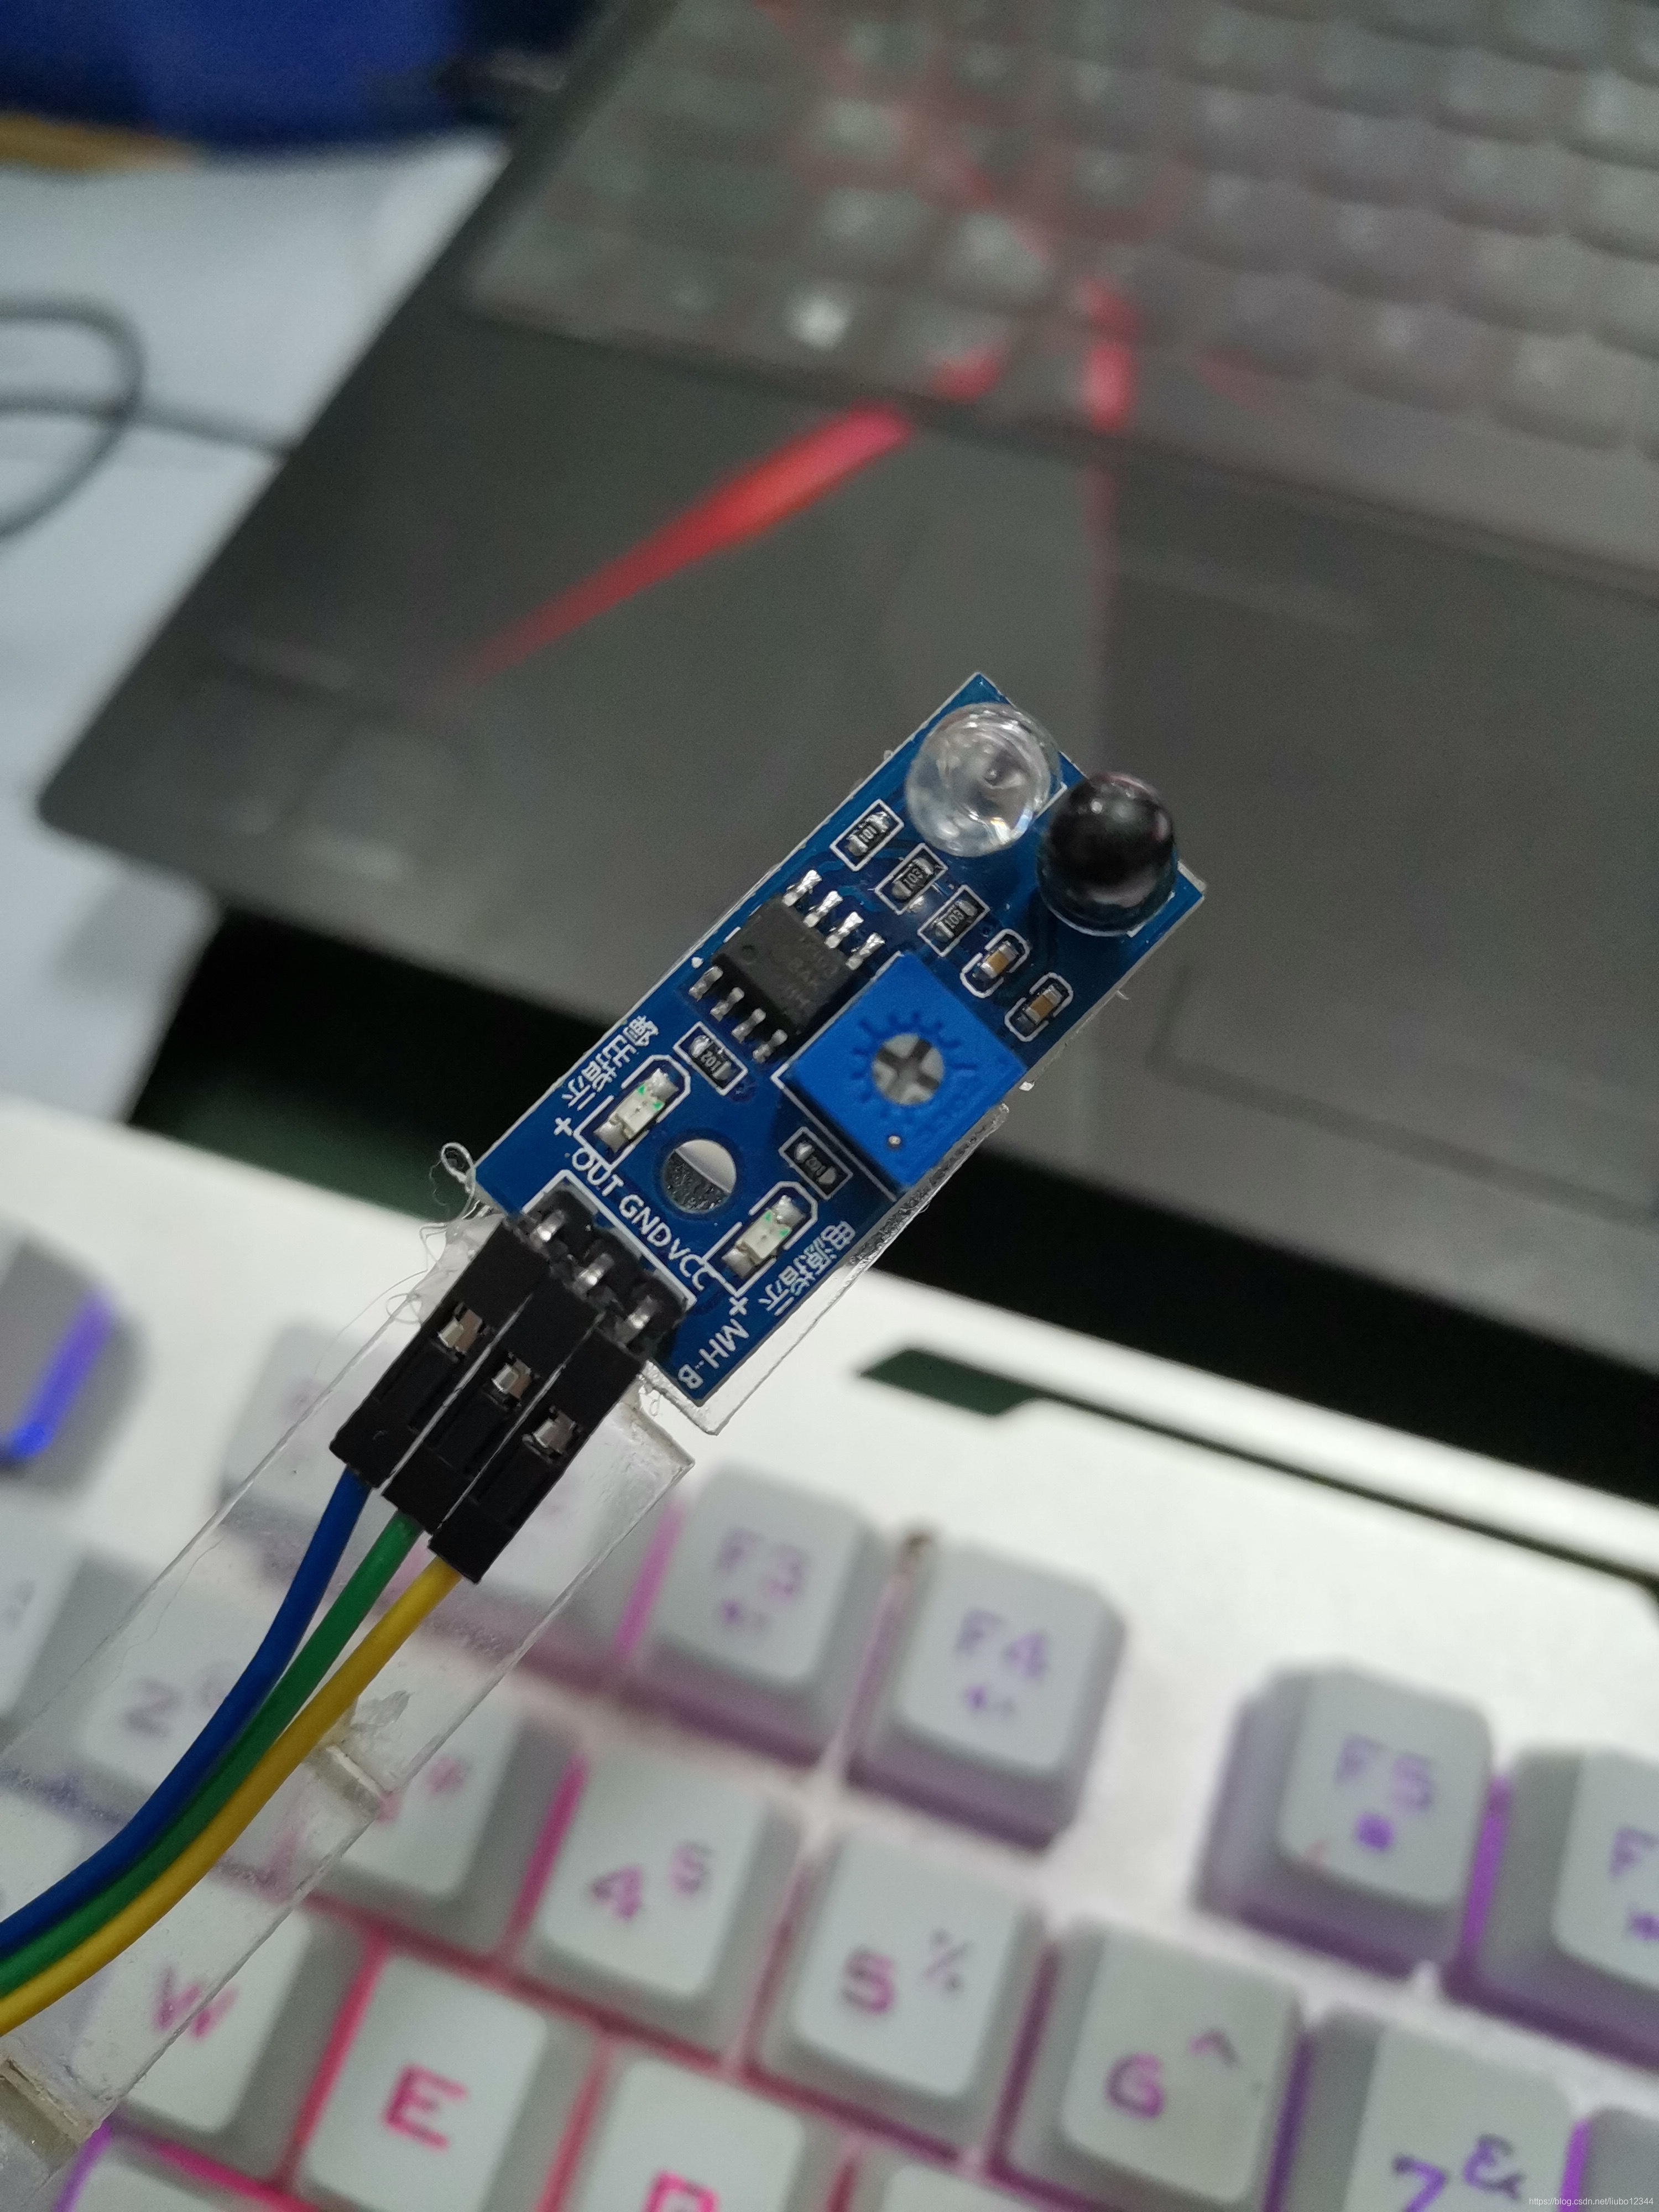
\includegraphics[width=0.5\textwidth]{figures/sensor.jpg}
  \caption{ 常见的红外传感器}
\end{figure}

常见的使用方案是在循迹车的前方布置对称的红外传感器。当线出现在红外传感器的正下方,它便会给控制电路采取行动的信号。例如当需要小车保持在黑色边线的赛道内时,如果侧边传感器有信号,则控制向另一个方向转弯。这种实现非常简单直观。

然而红外传感器的缺陷在于其只能给出是否检测到线的信息,而不能给出线的远近、角度信息,这使得它无法实现更加复杂和高效的控制算法。
\newpage
\subsubsection{算法:从if-else到PID}
\label{subsec:label}
空间上离散的点观测传感器实际上提供了有限的状态数,只要根据状态给定行为就可以完成简单的控制。这只需要简单的if-else逻辑就能实现。但这样简单的方法代价是不够灵活,并且一个固定的控制指令并不能总是实现最优的控制。实际上的小车可能会困在反复地左右摇摆中浪费大量的时间和能量。

如果我们有一个点观测传感器组成的阵列例如线性CCD(含有128个光敏电阻)或者进一步线性传感器,我们可以离散地或连续地得到与线之间的距离。如使用线性CCD元件\cite{CCD},将黑线在CCD正中间认为是基准值,数值从右向左增加,误差定义为当前值与标准值的差。这使得我们能够向循迹算法中引入PID。设定一个中间状态作为PID的基准,传感器阵列得到的距离可以作为PID的误差。利用PID控制两轮的转速差,使其小车保持在中间状态,可以实现更平滑、更快的循迹。

\subsection{更灵活高效的新方法}
\label{subsec:label}
\subsubsection{计算机视觉\cite{opencv}}
\label{subsec:label}
采用计算机视觉方法可以为系统获得更广的感受野和更复杂的信息。传统的方式是首先获取图像,把图像转化成灰度图再进行二值化,得到黑白图像。黑色点的平均横坐标反映了循迹线的倾斜程度。据此,可以设置阈值或PID使得小车保持循迹。
\begin{figure}[ht]
  \centering
   \begin{subfigure}[b]{0.3\textwidth}
     \centering
     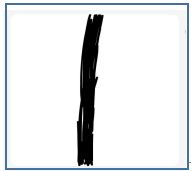
\includegraphics[width=\textwidth]{figures/straight.png}
     \caption{直行}
     \label{fig:label}
   \end{subfigure}
   \hfill
 \begin{subfigure}[b]{0.3\textwidth}
   \centering
   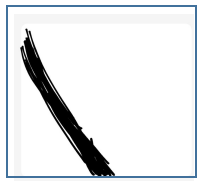
\includegraphics[width=\textwidth]{figures/left.png}
   \caption{左转}
   \label{fig:label}
 \end{subfigure}
 \hfill
 \begin{subfigure}[b]{0.3\textwidth}
   \centering
   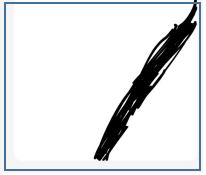
\includegraphics[width=\textwidth]{figures/right.png}
   \caption{右转}
   \label{fig:label}
 \end{subfigure}
 \hfill
  \caption{经过灰阶化-二值化的图像}
\end{figure}

但对于单片机而言,矩阵的高运算量带来的时间消耗限制小车的移动速度。这时我们就需要对算法进行优化。首先并不是视野中的所有信息都需要被纳入决策中,我们实际上只需要考虑距离小车较近的部分,可以裁剪掉多余的部分。接着,每一帧图像中黑线的趋势可以间隔采样来获取,而不是全部计算。卷积也可以有效地减小需要遍历的矩阵。采用矩阵池化来用局部特征替代整体特征。池化实际上是将矩阵分成多个与卷积核一样大的小块,使用小块内元素的特征(最大值或者平均值)来代替这个区域。
\begin{figure}[ht]
  \centering
 \begin{subfigure}[b]{0.4\textwidth}
   \centering
   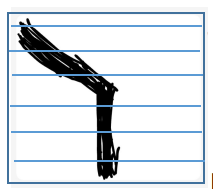
\includegraphics[width=\textwidth]{figures/jumpscan.png}
   \caption{间隔采样}
   \label{fig:label}
 \end{subfigure}
 \hfill
 \begin{subfigure}[b]{0.4\textwidth}
   \centering
   \includegraphics[width=\textwidth]{figures/pooling.png}
   \caption{最大值池化}
   \label{fig:label}
 \end{subfigure}
 \hfill

\end{figure}
\newpage
\subsubsection{强化学习}
\label{subsec:label}
2024年Yu Cao等人进行了深度强化学习循迹机器人的理论研究\cite{cao2024path}。他们将机器人与线路的横向偏差、机器人与路径之间的方向误差、机器人的速度和角速度等信息作为状态,而将机器人速度的变化率作为行动。在奖励函数中纳入与误差成正比的惩罚、与速度成正比的奖励以及惩罚机器人在困难弯道停下的参数。

\begin{figure}[ht]
  \centering
  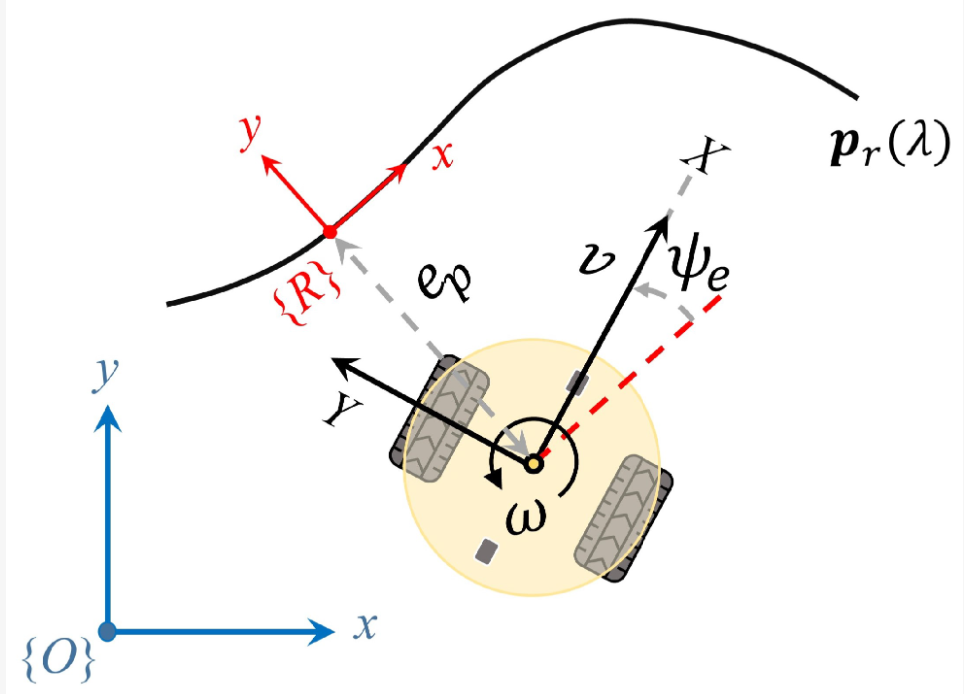
\includegraphics[width=0.5\textwidth]{figures/state.png}
  \caption{状态定义物理量\cite{cao2024path}}
\end{figure}

\[ r\left(t\right)=-k_{1}\left|e_{p}\left(t\right)\right|+k_{2}v\left(t\right)\left(1-\frac{1}{e_{tol}}\left|e_{p}\left(t\right)\right|\right)-k_{3}F\left(t\right) \]

在随机生成的环境中进行了50万次交互之后,机器人的路径实现收敛。相比传统的PP控制方法,采用深度强化学习的机器人有了自适应的速度控制能力,可以适应不同曲率的路径,还有相当不错的泛化能力,在随机生成的不同路径中均有优秀的效果。

根据现实硬件情况在Webbot中建模并进行虚拟环境的预训练,再将完成训练的模型下载到实际小车中,就可以实现该方法的实际运用。
\section{避障研究综述}
\label{sec:label}
\subsection{需要获取的信息和相关传感器}
\label{subsec:label}
\subsubsection{障碍物信息}
\label{subsec:label}
\paragraph{红外避障传感器}

原理:红外传感器有一对红外发射管和接收管。发射管发射出一定频率的红外线,当检测方向遇到障碍物时,红外线会反射回来被接收管接收。当正前方有障碍物时,输出低电平;在一定范围内没有障碍物,则返回高电平。

红外传感器的测距原理是三角测距,其特点为白色物体反射的最远距离较大;黑色物体反射的最远距离较小,但无法检测透明的或近似黑体的物体;面积大的物体所能探测的距离大,面积小的物体所能探测的距离小;可以同时检测偏移角为40°的物体,带宽高于超声波。值得一提的是,当D的距离足够近的时候,上述L值会相当大,可能会超过CCD的探测范围;当D的距离很大的时候,L值会变小,测量精度会变差\cite{jh1}。
  \begin{figure}[ht]
    \centering
    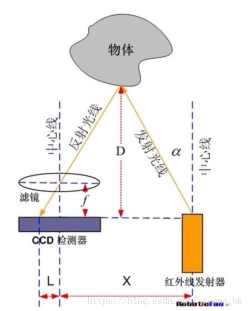
\includegraphics[width=0.5\textwidth]{figures/hongwaibizhang.png}
    \caption{红外避障原理 }
  \end{figure}
\newpage
  \paragraph{超声波传感器}
  
原理:超声波传感器主要材料为压电晶体和镍铁铝合金两类。压电晶体组成的超声波传感器是可逆的,可以将电能转化为机械能产生超声波;接受到超声波之后也可以转化成电能。

超声波波长短、频率高、绕射现象小、方向性好。在传感器中,超声波的发射器将产生机械震荡,发出超声波;超声波遇到被测物体后,会引发反射/折射,由接收器接受回波,转换成电信号处理。超声波波速已知,只需根据发射和接收的时间差,就可以计算出测量距离;结合发射器和接收器的距离,就可以算出障碍物的实际距离。

超声波的传感器成本低、实现方法简单、技术成熟,在比较精确的测量中,需要考虑温、湿度变化和其他因素。超声波传感器一般作用距离较短,普通的有效探测距离是米级,但是会有十毫米级的探测盲区。因为超声波是锥形传播的,其探测到的是某个锥形角度范围内最近物体的距离。超声波传感器的劣势在于测距时间较长,感应精度较低,容易受到其他超声传感器的干扰,会出现较多噪点。
  \begin{figure}[ht]
    \centering
    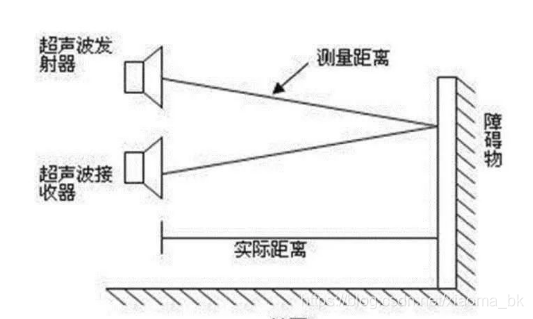
\includegraphics[width=0.5\textwidth]{figures/super.png}
    \caption{超声波测距原理 }
  \end{figure}

  \paragraph{激光雷达}
  
原理:发射激光然后接受,可以类似红外激光进行三角测量,也可以类似超声波进行时间差+速度测量。激光雷达包括发射器和接收器,发射器用激光照射目标,接收器接受返回的光波。机械式的激光雷达包括一个带有镜子的机械机构,镜子的旋转使光束可以覆盖一个平面 ,如此可以得到一个平面上的距离信息。

测量方案:主流的方案有两种,一种是基于飞行时间测量(TOF),一种是三角测距。TOF的基础公式是 \( d=\frac{ct}{2} \),其中时间t的测量是相对核心的环节,主要有以下三种方法:第一种是直接测量,使用脉冲激光直接测量占用的时间,但是因为光速远高于声速,对时间测量元件的精度要求较高,因此价格昂贵;第二种是差频测量,发射调频后的连续及广播,通过测量接收到的反射波之间的差频测量时间;第三种是相移测量,传感器以已知的频率发射一定幅度的调制光,并测量发射和反向信号间的相移,根据调制波信号的波长和相移即可获得距离。

三角测距原理则和红外测距一样,此处不再赘述。

激光雷达测距的特点是测量距离的置信度反比于接收信号幅度的平方,角度分辨率高,测距精度高;但是远距离物体和黑体的距离测量不容易估计,透明材料不易估计;成本高,价格较贵;三角测距雷达的量程会受到限制,一般在几米以内,而且精度相对较低\cite{jh1}。
\newpage
  \paragraph{毫米波雷达}
  
 毫米波雷达是通过毫米波段的电波测量距离、相对距离、方向等的雷达传感器。在行驶过程中向前方发射毫米波段的点播,若前方有障碍,则可收到反射回来的回波。通过分析监测到的反射波频率变化(即发射频率和接收频率的差值),检测前方及对面是否有障碍、与前方及对面障碍间的距离、相对速度和方向等。
基本原理同上述雷达,但是也有一些特性:毫米波雷达检测距离较长;金属表面和夜间、逆光、雾、雨、雪环境下也能使用;非金属表面反射不佳,检测困难(如人、纸箱等)。因此,毫米波雷达不作为本次实验的预选方案\cite{jh2}。

  \subsubsection{位置信息}
  \label{subsec:label}
为了实现精确的算法,需要收集必要的位置信息,以确定小车当前所处位置以及小车已完成的路程。位置信息可以用矢量表示,因此需要一个角度信息和一个距离信息,分别由陀螺仪和里程计两种传感器测量并提供。

\subsection{避障算法}
\label{subsec:label}
智能车作为一种具有自主决策能力的机器人,需要从外部获取环境信息并作出决策,从而做出全局路径规划和局部危险状况下的避障。全局规划为智能车提供了已知地图环境下的最优路径,而局部危险状况避障则有利于智能车对不可预测的事件及时做出反应,以求顺利到达目的地并完成任务。因此,局部避障算法必须速度快、实时性好且效率高,并承担智能车避障的主要工作。接下来将就全局规划算法和局部避障算法分别进行介绍。

\subsubsection{全局规划算法}
\label{subsec:label}
全局规划算法是在全局地图已知(至少是起点和终点已知)的情况下规划出的最优路径,主要目的是节省时间,提高效率。下文总结了目前的部分全局规划算法。
\paragraph{A*算法}
A*算法最早发表于1968年,是Dijkstra算法和广度优先搜索算法(BFS)的结合体,利用启发式函数f(n)=g(n)+h(n)快速找到最优路径。

函数中,f(n)标识节点的综合优先级函数,选择结点时考虑该节点的综合优先级(总成本);g(n)表示起始点到点n的实际成本;h(n)标识当前节点到目标点的代价估值函数(预估成本),即当前位置n到达目的地的最佳路径的启发值,需要通过事先设计来满足实际的地形或环境特征。理想情况下,h(n)不会高于实际的成本,这样才能满足找到的是最低成本路径。

三个函数定义如下:
\begin{enumerate}
\item 	h(n)(启发式函数-代价估值函数):对于网格点(x,y),目标点($x_0$,$y_0$),启发式函数可以如此定义: \( h(n)=\sqrt{(x-x_0)^2+(y-y_0)^2} \) 这个函数值实际上是当前点到重点的欧里几得距离。
\item $g(n)$ (成本函数) :每当从起始点通过路径移动到一个新节点,$g(n)$需要累加上到达该节点的移动成本。设每一步的移动成本是w,则:$g(n_{next})=g(n_{now})+w$
  \item  $f(n)$(总成本):综合上述值,得到$f(n)$评价总成本,最终从中选取节点$f(n)=g(n)+h(n)$

  \end{enumerate}
  \newpage
A$^{*}$算法尽管有着一定的高效、灵活和普适性,但仍然有不少的问题。启发式函数$h(n)$的选择会高度影响 A$^\star$算法的准确性,若不合适可能会导致找不到解或搜索效率低下;A*算法需要维护开放列表和封闭列表,存储大量的节点信息,会消耗大量内存;动态变化环境中,A$^{*}$ 算法需要不 断重新计算,可能会影响其实时性能;在图特别大的情况下,A$^{*}$可能因为评估节点过多导致计算量较大和速度较慢。针对这些问题,陈鑫鹏等提出了等步长分层拓展的算法来改善\cite{jh3}。

\paragraph{$D^{*}$算法}

D*算法,又称动态A*算法,基于A*算法发展而来,最早用于火星探测器的寻路算法。

和A*算法从起点到终点的正向搜索不同,D*算法的搜索是从终点到起点,利用以前的搜索结果信息再利用实现高效搜索,大大减少搜索范围和时间适合面对周围环境未知或存在动态变化的场景。只需要假设地图开始没有任何障碍,起点到终点的路径为直线,在线运行时不断重新规划,即可完成全地图未知的路径规划。

对于D*算法,秦旭等对传统D*算法进行了改进,优化子节点的选取方式,同时改进代价估计函数并引入平滑度函数,规划时间节约了20\%;张希闻等提出了拓展Moore型元胞结构,对原D*算法的路径进一步缩短,将八点拓展到十六点,拥有更快的速度和更高的空间复杂度\cite{jh4}。
\paragraph{遗传算法}

遗传算法(GA)是John holland 在20世纪70年代初提出的根据生物体进化规律而设计的\cite{jh5}。它是一种全局最优解搜索的启发式优化算法,机制是模拟达尔文进化理论和自然界优胜劣汰。算法流程如下:
\begin{figure}[ht]
  \centering
  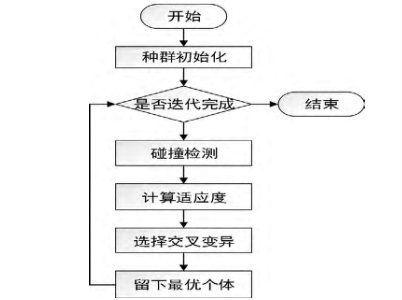
\includegraphics[width=0.5\textwidth]{figures/yichuan.png}
  \caption{遗传算法}
\end{figure}
\newpage
\paragraph{蚁群算法}

由Marco Dorigo 在1992年提出,是一种用于寻找优化路径的随机搜索算法\cite{jh5}。思路是将城市与城市之间的路径看作一幅图,放置n只蚂蚁在图中移动。每只蚂蚁成功到达终点的路径上会留下信息素,信息素最大的部分就是最优路径
\begin{figure}[ht]
  \centering
  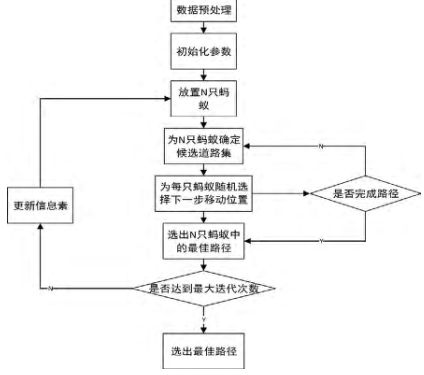
\includegraphics[width=0.5\textwidth]{figures/yiqun.png}
  \caption{蚁群算法 }
\end{figure}

\subsubsection{局部避障算法}
\label{subsec:label}
局部避障算法属于动态规划,主要信息来源是无人车传感器提供的环境信息。此种算法的设计目的是为了让机器人能够灵活调整决策,并尽快对路径上的算法做出响应,根据特点可以分为采样方法、条件约束法和机器学习法。常用的局部路径算法包括人工势场法和虚拟力场法。
\paragraph{人工势场法\cite{jh6}}

人工势场法(APF)是一种虚拟力法,它的思路是将车辆在周围环境中的运动视为车辆在人工建立的虚拟力场中的运动。目标点产生引力,引导车辆向目标点运动;障碍物产生斥力,避免车辆与障碍物相撞。车辆在二者的合力下运动,根据引力和斥力的合力控制车辆向势场下降的方向运动,产生一条无碰撞的最优路径。下文详细介绍引力、斥力的计算方式以及合力的计算公式。

引力势场主要与汽车和目标点之间的距离有关。距离越大,汽车所受的势能值就越大;距离越小,汽车所受的势能值就越小。因此,引力势场的函数是:
$$U_{att}(q)=\frac12\eta\rho^2(q,q_g)$$

其中$\eta$是正比例增益系数,$\rho(q,q_g)$是一个矢量,标识汽车的位置$q$和目标点位置$q_g$之间的欧式距离$|q-q_g|$,矢量方向是从汽车的位置指向目标位置,相应的引力$F_att(q)=-\nabla U_{att}(q)=-\eta\rho(q,q_g)$,是引力场的负梯度,代表引力势场函数$U_att(q)$变化最快的方向。
\newpage
决定障碍物斥力势场的因素是汽车与障碍物之间的距离。当汽车没有进入障碍物的影响范围时,其受到的势能为 0;汽车进入障碍物影响范围后,汽车受到的势能与距离的关系呈负相关。设车辆当前和目标点的距离为$\rho_g^n$,其中$n$自行定义。具体公式如下:
$$U_{req}(q)=\begin{cases}\dfrac{1}{2}k\left(\dfrac{1}{\rho(q,q_g)}-\dfrac{1}{\rho_0}\right)\rho_g^n,&\quad0\leq\rho(q,q_g)\leq\rho_0,\\\\0\:,&\quad\rho(q,q_g)>\rho_0\end{cases}$$
$F_{req1}$方向为障碍物指向车辆;$F_req2$方向为车辆指向目标点;$F_req$为斥力势场的负梯度作用力。即斥力势场的负梯度作用力等于障碍物指向车辆的斥力和车辆到目标点的斥力之和。
\begin{align}
  \label{}
F_{req}&=F_{req1}+F_{req1}\\
F_req1&=k\left(\frac1{\rho(q,q_g)}-\frac1{\rho_0}\right)\frac{\rho_g^n}{\rho^2(q,q_g)}\\
F_req2&=\frac n2k\left(\frac1{\rho(q,q_g)}-\frac1{\rho_0}\right)^2\rho_g^{n-1}
\end{align}
\begin{figure}[ht]
  \centering
  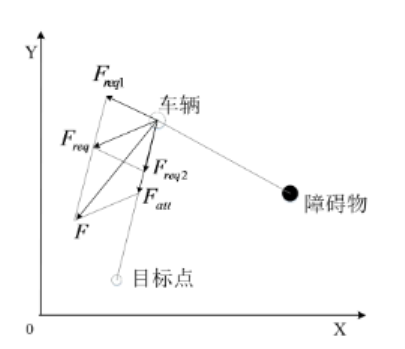
\includegraphics[width=0.5\textwidth]{figures/APF.png}
  \caption{车辆在改进后势场中的受力}
\end{figure}

根据上述定义的引力场和斥力场函数,可以得到整个空间的复合场,机器人合力势场大小为机器人所受斥力势场和引力势场之和,故合力势场总函数是:
\[ U(q)=U_{att}(q)+U_{req}(q) \]
所受合力是:
\[ F(q)=-\nabla U(q)=F_{att}(q)+F_{req}(q) \]
合力方向决定汽车的行驶朝向;合力大小决定汽车的行驶加速度。
\newpage
应用人工势场法规划出来的路径一般比较平滑安全、算法简明,实时性良好。但是算法也有一些缺点:
\begin{enumerate}
\item 当目标点附近有障碍物时,斥力远远大于引力,车辆将很难到达目的地。
\item 当智能车在某一点引力和斥力刚好大小相等时,车辆会陷入局部最优点。
\item 当车辆到达障碍物附近时,人工势场模型产生的轨迹将出现抖动,不光滑\cite{jh8}。
\item 当引力过大时,即无人车位于起始位置时,无人车可能会忽略障碍物斥力的作用造成碰撞\cite{jh7}。
  \item 传统人工势场只考虑了障碍物与目标点静止不动的静态环境,而车辆实际是在运动的环境中,因此在动态环境下无法取得良好的效果。
\end{enumerate}
针对这些问题,学界产生了很多改进措施。

王会丽等改进势场函数,解决局部最优点问题,成功找到全局最小点;李钧泽等对引力和斥力做了改进,有效解决了与原目标端障碍物相撞和目标点不可达的问题,引入临时障碍物有效解决了局部极小值问题;余震中等使用势场强度代替力矢量进行路径规划,在障碍物斥力市场中添加系数项,解决障碍物与目标点过近导致目标不可达的问题;考虑移动速度与机器人速度影响,引入速度信息,解决了动态环境下移动机器人的路径规划\cite{jh5}。

\paragraph{模糊逻辑算法}

模糊逻辑算法是一种常用的在线路径规划算法,一般先建立模型,再进行局部路径规划。该算法根据观摩和记录驾驶员的操作过程得到,无需针对特定对象建立相关数学模型,而是直接将驾驶员的驾驶经验转换成相关控制信号。车辆在进行避障路径规划的过程中,将获得的环境信息模糊化,通过不断查找相关的模糊规则获得规划结果。还有学者建立了动态模糊环境模型,将环境中运动物体的运动状态用模糊集标识,包括运动物体当前位置、速度大小和方向等,之后利用模糊规则对各个方向进行综合评价以得到搜索结果。
模糊算法不需要车辆精确定位,所以具有很高的鲁棒性,对各种未知情况适应性较好,路径规划效果良好,但是模糊算法不能自我学习,模糊规则指定后就一成不变,灵活性较差\cite{jh6}。

\chapter{原型设计方案}

\section{机械设计}
\subsection{车体}
\label{subsec:label}
车体的驱动机构我们计划采用两个前轮驱动轮+一个后轮万向轮的结构,因此车体构型接近倒三角型。纵向上采用双层结构,下层搭载电机、电池、机械夹爪和舵机等,上层搭载各个控制硬件和通信硬件,包括STM32、电压转换模块、蓝牙模块和超声波传感器等。为了让OpenMV工作效果更好,将其放置到更高的位置上,便于增加观测距离。
\begin{figure}[ht]
  \centering
  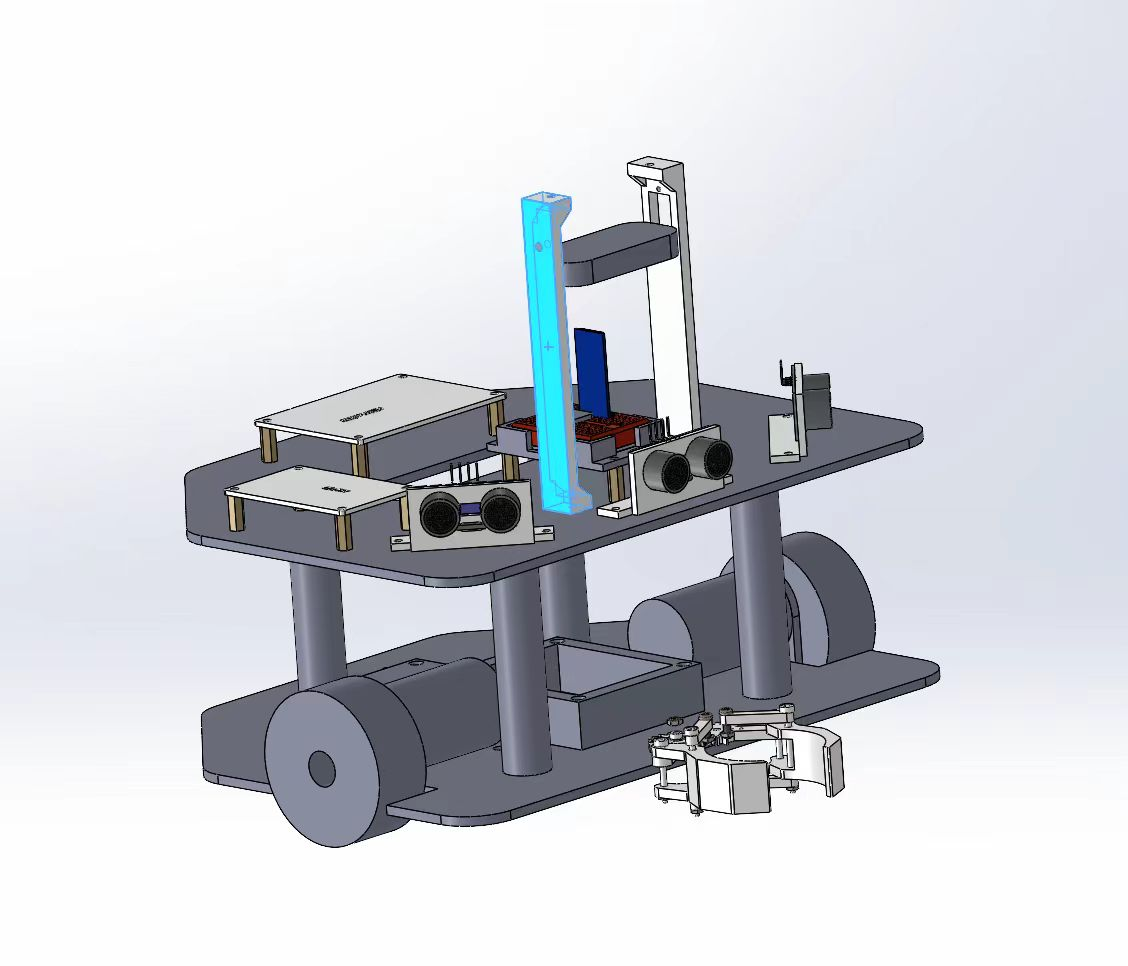
\includegraphics[width=0.5\textwidth]{figures/body.jpg}
  \caption{车体原型}
\end{figure}

\subsection{抓取机构}
抓取机构既需要满足摩擦力的需求,能够稳定地夹取物体;同时又不能太大,避免遮挡传感器干扰其正常工作。综合考虑以上要求,在机械夹爪、吸盘和仿生结构中我们最终选择了单自由度的机械夹爪结构。利用电机转动带动齿轮转动从而带动机械夹爪转动,使得一个电机能够同时驱动两侧夹爪转动。夹爪的上面和下面各有一对连杆进行固定和限位,并使用螺栓螺母等零件加固,保证夹取机构的稳定性。
\begin{figure}[ht]
  \centering
  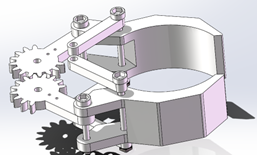
\includegraphics[width=0.5\textwidth]{figures/pickup.png}
  \caption{抓取机构概念图 }
\end{figure}
\newpage
\section{测量}
\label{sec:label}
\subsection{小车位姿测量}
\label{subsec:label}
为了对小车进行定位以及进行下一步的计算,我们需要对小车的位姿进行测量。综合考虑各种传感器的性能之后,我们初步决定采用从动轮+里程计的方式测量小车移动的距离,用陀螺仪测量小车转过的角度,从而确定小车的位姿。
\subsection{循迹中的测量}
\label{subsec:label}
由于我们计划采用视觉循迹方案,所以需要实时图像等视觉数据。我们计划采用OpenMV视觉传感器,其具备计算处理能力,有利于提高图像处理帧率,同时封装性良好,便于我们在短时间内快速学习并应用。
\subsection{避障中的测量}
\label{subsec:label}
我们计划采用激光测距传感器获取距离信息为主,辅以OpenMV视觉传感器进行目标识别。如此可以充分利用OpenMV获得的二维图像信息与较好的前瞻性,并用激光测距测量小车其他方向距障碍物的距离作为补充,并且通过随机算法与人工势场法的加权实现小车前进方向的实时更新,之后会在实现中具体论证可行性。
\section{循迹}
\label{sec:label}
我们选择使用视觉循迹方案。文献综述中包括了点传感器(红外传感器和光敏电阻)、线性CCD、视觉循迹和强化学习循迹四种方案。点传感器方案只有离散的极少状态,控制算法设计空间小,循迹的平滑性和速度都不够令人满意。CCD实际上是一个点传感器的阵列,信息获取精度仍然较低,前瞻性较有限。而强化学习方案要求更加复杂的环境感知能力,并且需要在虚拟环境中进行大量的预训练才能得到收敛的路径,实现难度大,我们现有的笔记本电脑显卡算力有限,因此不作为优先选择。
\subsection{视觉传感器选择}
\label{subsec:label}
视觉传感器选型方面,我们将使用OpenMV。OpenMV的优势在于其本身是一个单片机,具备计算处理能力,有利于提高图像处理帧率,提高小车整体性能。另外,OpenMV配套开发工具封装良好,官方文档详细,开放资源丰富。这对于开发者而言无疑是能大大降低学习成本、提高效率的。
\subsection{算法选择}
\label{subsec:label}
整体而言,我们的算法是先进行图像预处理再加入PID控制。

我们会利用OpenMV自带的二值化工具将裁剪后的图像转化成黑白图像。然后,选取视场中中间靠前的区域作为ROI进行裁剪或矩阵池化来缩小矩阵。接着,用OpenMV自带的拟合函数计算出黑线方程。根据黑线斜率给出转向控制量。控制量的产生需要经过PID来保持稳定平滑。需要注意,PID的误差量是黑线斜率和基准斜率的差距,而控制量是两轮之间的转速差。
\section{避障算法设计}
\label{sec:label}
\subsection{避障信息获取}
\label{subsec:label}
\subsubsection{位置信息}
\label{subsec:label}
避障需要小车找到自身所处的位置和方向,因此需要生成车辆的矢量路径。矢量路径有两个关键信息:角度和距离。角度信息预计使用陀螺仪记录小车当前方位与初始方位的夹角,距离信息使用里程计模块记录距离。

使用陀螺仪记录小车当前方位与初始方位的夹角。当陀螺仪记录角度在任意一侧超过90度且行走距离超过当前总距离的一定比例时,停止前进,原路返回。

使用里程器模块记录距离。使用编码器记录主动轮转动的圈数,并通过一系列公式将圈数转换为当前方向上走过的距离并记录。

\subsubsection{障碍物信息}
\label{subsec:label}
避障需要找到障碍物的位置。我们预计是使用超声波雷达获得与障碍物的距离信息。我们预计采用人工势场法,因此只需要识别前方已有的障碍物并给出当前距离即可收集障碍物信息。
\subsection{避障算法设计}
\label{subsec:label}
避障预期采用人工势场法。依据文献调研结果,结合小车所处的环境状况,预计对人工势场法作出以下改进:
\subsubsection{数学模型改进}
\label{subsec:label}
根据文献调研,人工势场法在使用过程中会出现一些问题,如因障碍物和终点距离太近导致已经到达势能零点、出现局部最优点等。针对这些问题,将数学模型更新如下。

根据梅艺林等人在2024年的工作\cite{jh7},引力势场的数学模型可以更新成如下形式:
\[ U_{att}(q)=k\frac1{\left(1+e^{\delta\Delta\rho(q,q_g)}\right)^2}+\alpha\Delta\rho(q,q_g) \]

对其求负梯度,改进引力场计算公式:

\[ F_{att}(q)=-\omega\frac{e^{\delta\Delta\rho(q,q_g)}}{\left(1+e^{\delta\Delta\rho(q,q_g)}\right)^2}+\alpha  \]
其中$\omega$引力增益系数,$\delta$是引力变化范围调节因子,$\alpha$是引力上下限调节因子。

改进的斥力势场公式如下:
\[ U_{req}(q)=k\Delta\rho(q,q_g)-k\frac{\ln{(e^{\eta\Delta\rho(q,q_g)}+1)}}{\eta} \]
对其求负梯度,改进斥力场计算公式:
\[ F_{req}(q)=k\frac1{1+e^{\eta\Delta\rho(q,q_g)}} \]
其中k是斥力大小系数,$\eta$是斥力作用范围调节因子,$\Delta\rho(q,q_{g})$是与$\rho(q,q_{g})$相关的调节因子
\subsubsection{思路改进}
\label{subsec:label}
首先,将终点所在直线设定为一级引力场,促使小车不断向最远端行进,以此避免小车可能出现的折返问题;当到达一级引力场时,旋转小车角度与引力场直线方向一致,并向前行进,如果摄像头在地面上识别到终点圆圈,进行放置的步骤;如果摄像头到达墙后仍没有终点圆圈,旋转180度,回到一级引力场,重新向前遍历。

\section{数据通信和回传}
\label{sec:label}
\subsection{蓝牙模块}
\label{subsec:label}
基于我们的场景中通信距离短、有抗干扰需求的情况,我们选择使用蓝牙模块实现通信。蓝牙模块有着体积小、易集成、功耗低的特点,对于板载设计友好。蓝牙通信协议的跳频-扩频机制提供了很好的抗干扰能力。2.4G的电磁波可以穿过大多材料的障碍物,利于小车行驶时仍然保持与控制终端的稳定信息交换。实际预计采用蓝牙模块HC-05。HC-05相关资料多,配套开发工具丰富,学习使用便捷。HC-05具备全双工能力,可以实现可靠的信息互传。我们将通过电脑或手机向HC-05传输指令,再有HC-05控制单片机并返回传感信息。
\begin{figure}[ht]
  \centering
  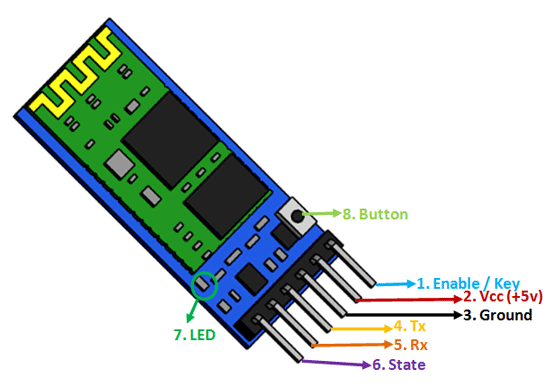
\includegraphics[width=0.5\textwidth]{figures/hc-05.png}
  \caption{\label{fig:label} }
\end{figure}
\newpage
\subsection{控制终端}
\label{subsec:label}
为了便于控制和调试,我们计划通过蓝牙传输的方式将数据传回PC端进行观察和控制,可以通过编码器数据得知车轮转过的里程数,通过陀螺仪确定小车转过的角度。此外,还可以通过蓝牙模块在PC终端对小车进行控制,比如紧急停车和转向等,方便在小车出现问题的时候观察出现问题的模块,从而进行针对性的改变和调试,提高调试效率。
\begin{figure}[ht]
  \centering
  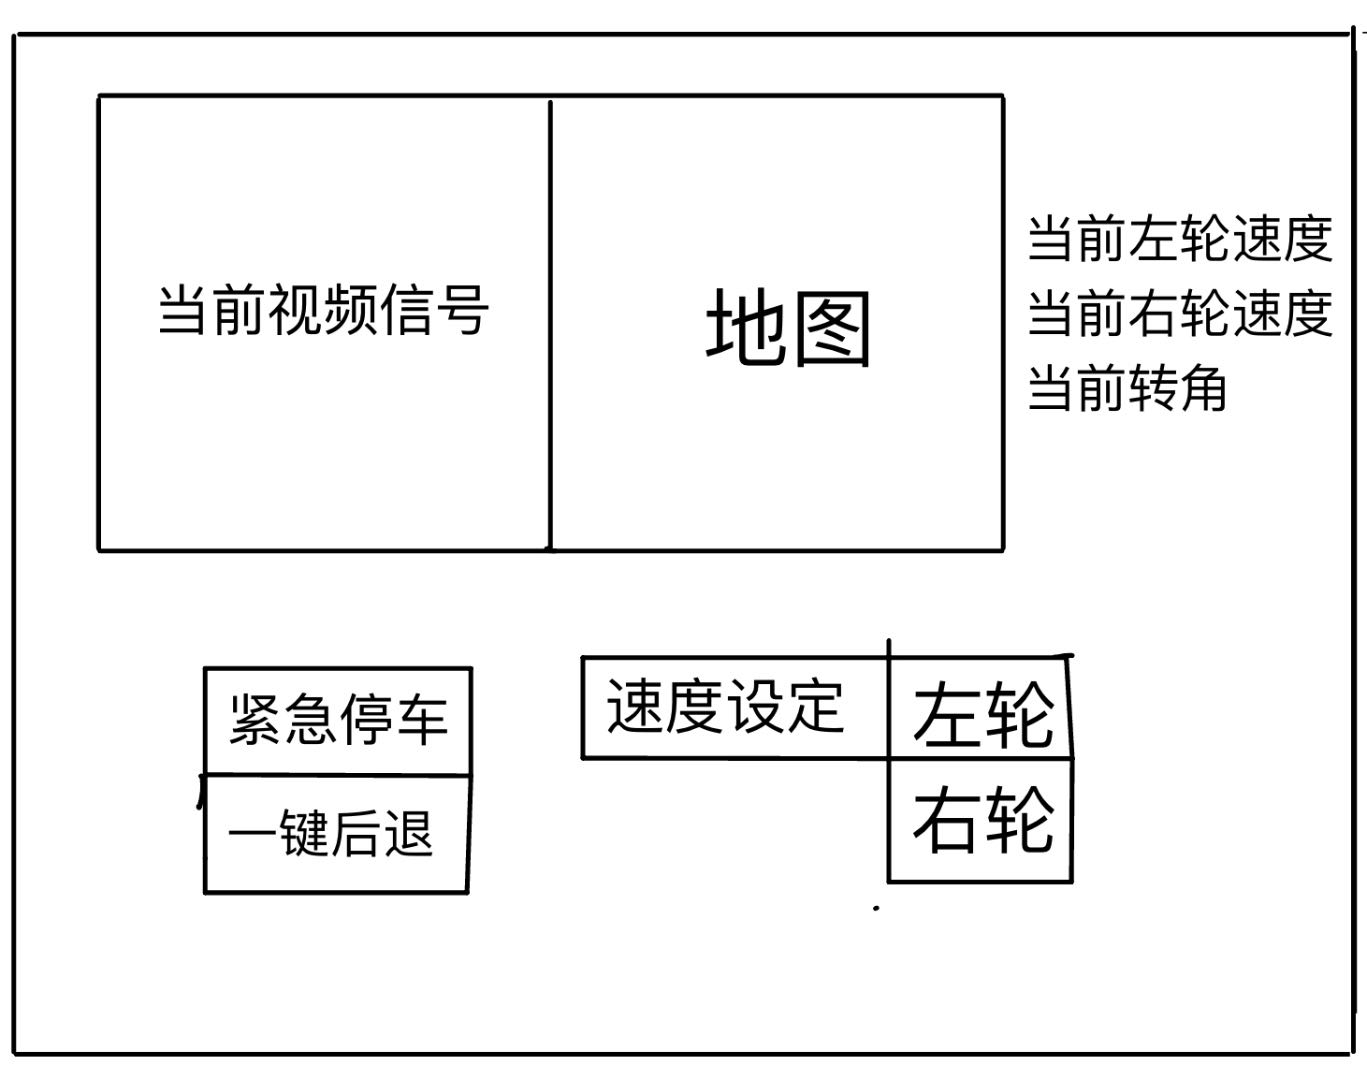
\includegraphics[width=0.5\textwidth]{figures/ui.jpg}
  \caption{控制终端UI概念图 }
\end{figure}


\section{驱动}
\label{sec:label}
\subsection{处理器}
硬件的选取需要同时考虑设计需求和实际运算能力。FPGA的并发速度快,可靠性好,但调试困难,其他传统形式则难度更大,相比之下,采用CPU会简便许多。对于整个算法中最重要的图像处理部分,已有的STM32具有足够的数据处理能力。由于本组同学使用树莓派单片机的经验较少,考虑到本课程的任务进度要求,我们决定不使用树莓派单片机,而是选用OpenMV进行图像处理方面的数据。综上,我们初步计划采用STM32为主、OpenMV为辅的处理器组合。

\label{subsec:label}
\subsection{电机驱动}
\label{subsec:label}
选择使用PWM方法驱动,并用编码器回传电机数据。选择L298模块同时驱动两轮电机,并使用PID实现电机实际速度的准确、稳定控制。
\subsection{传感器}
\label{subsec:label}
\begin{enumerate}
\item OpenMV:自带单片机,不需要额外的驱动元件。
\item 超声波传感器:可以使用UART串口通信。
\item 里程计:里程计实际上是一个主动轮电机上的编码器,因此不需要进一步的驱动元件。
  \item 陀螺仪:不需要额外的驱动元件,使用$I^{2}C$通信。

  \end{enumerate}
  \newpage
\section{硬件清单}
\label{sec:label}
% Please add the following required packages to your document preamble:
% \usepackage{multirow}
% \usepackage{graphicx}
% \usepackage[table,xcdraw]{xcolor}
% Beamer presentation requires \usepackage{colortbl} instead of \usepackage[table,xcdraw]{xcolor}
% Please add the following required packages to your document preamble:
% \usepackage{multirow}
% \usepackage{graphicx}
% \usepackage[table,xcdraw]{xcolor}
% Beamer presentation requires \usepackage{colortbl} instead of \usepackage[table,xcdraw]{xcolor}
\begin{table}[ht]
\centering
\resizebox{0.5\textwidth}{!}{%
\begin{tabular}{|
>{\columncolor[HTML]{FFFFFF}}c |
>{\columncolor[HTML]{FFFFFF}}c |
>{\columncolor[HTML]{FFFFFF}}c |}
\hline
\textbf{类别}                                   & \textbf{名称/型号}   & \textbf{数量} \\ \hline
处理器                                           & CPU/STM32f407ZGT & 1           \\ \hline
\cellcolor[HTML]{FFFFFF}                      & OpenMV           & 1           \\ \cline{2-3} 
\cellcolor[HTML]{FFFFFF}                      & 超声波雷达           & 3           \\ \cline{2-3} 
\cellcolor[HTML]{FFFFFF}                      & IMU      & 1           \\ \cline{2-3} 
\multirow{-4}{*}{\cellcolor[HTML]{FFFFFF}传感器} & 里程计(用编码器实现)             & 1           \\ \hline
通信                                            & 蓝牙模块/HC-05       & 1           \\ \hline
\cellcolor[HTML]{FFFFFF}                      & 电机 (含直流电机和舵机)           & 3           \\ \cline{2-3} 
\cellcolor[HTML]{FFFFFF}                      & 电机驱动器/L298         & 2           \\ \cline{2-3} 
\multirow{-3}{*}{\cellcolor[HTML]{FFFFFF}动力}  & 电机上编码器              & 3           \\ \hline
\cellcolor[HTML]{FFFFFF}                      & 主动轮              & 2           \\ \cline{2-3} 
\multirow{-2}{*}{\cellcolor[HTML]{FFFFFF}车轮}  & 万向轮              & 1           \\ \hline
\end{tabular}%
}
\caption{}
\label{tab:my-table}
\end{table}


\bibliographystyle{IEEEtran}
\bibliography{references}

\end{document}

%%% Local Variables:
%%% mode: LaTeX
%%% TeX-master: t
%%% End:
